% LaTeX source for textbook ``How to think like a computer scientist''
% Copyright (c)  2001  Allen B. Downey, Jeffrey Elkner, and Chris Meyers.

% Permission is granted to copy, distribute and/or modify this
% document under the terms of the GNU Free Documentation License,
% Version 1.1  or any later version published by the Free Software
% Foundation; with the Invariant Sections being "Contributor List",
% with no Front-Cover Texts, and with no Back-Cover Texts. A copy of
% the license is included in the section entitled "GNU Free
% Documentation License".

% This distribution includes a file named fdl.tex that contains the text
% of the GNU Free Documentation License.  If it is missing, you can obtain
% it from www.gnu.org or by writing to the Free Software Foundation,
% Inc., 59 Temple Place - Suite 330, Boston, MA 02111-1307, USA.

\chapter{Listas}
\index{lista}
\index{elemento}
\index{secuencia}

Una {\bf lista} es un conjunto ordenado de valores que se identifican
por medio de un índice.  Los valores que componen una lista se 
denominan  {\bf elementos}. Las listas son similares a las cadenas, 
que son conjuntos ordenados de carácteres, pero son mas generales, ya
que pueden tener elementos de cualquier tipo de dato. Las listas y 
las cadenas---y otras conjuntos ordenados que veremos--- se denominan 
{\bf secuencias}.


\section{Creación de listas}

Hay varias formas de crear una nueva lista; la más simple es
encerrar los elementos entre corchetes (\verb+[+ y \verb+]+):

\beforeverb
\begin{verbatim}
[10, 20, 30, 40]
["correo", "lapiz", "carro"]
\end{verbatim}
\afterverb
%
El primer ejemplo es una lista de cuatro enteros, la segunda, una
lista de tres cadenas. Los elementos de una lista no tienen que
tener el mismo tipo. La siguiente lista contiene una cadena, un 
flotante, un entero y (mirabile dictu) otra lista:

\beforeverb
\begin{verbatim}
["hola", 2.0, 5, [10, 20]]
\end{verbatim}
\afterverb
%
Cuando una lista está contenida por  otra  se dice que está {\bf anidada}.

\index{lista!anidada}

Las listas que contienen enteros consecutivos son muy comunes, así que
Python proporciona una forma de crearlas:

\beforeverb
\begin{verbatim}
>>> range(1,5)
[1, 2, 3, 4]
\end{verbatim}
\afterverb
%
La función  \texttt{range} toma dos argumentos y retorna una lista
que contiene todos los enteros desde el primero hasta el segundo,
¡incluyendo el primero y no el último!

Hay otras formas de usar a  \texttt{range}.  Con un solo argumento
crea una lista que empieza en  0:

\beforeverb
\begin{verbatim}
>>> range(10)
[0, 1, 2, 3, 4, 5, 6, 7, 8, 9]
\end{verbatim}
\afterverb
%
Si hay un tercer argumento, este especifica el espacio entre los
valores sucesivos, que se denomina el  {\bf tamaño del paso}.  Este 
ejemplo cuenta de  1 a 10 con un paso de tamaño 2:

\beforeverb
\begin{verbatim}
>>> range(1, 10, 2)
[1, 3, 5, 7, 9]
\end{verbatim}
\afterverb
%
Finalmente, existe una lista especial que no contiene elementos. Se 
denomina lista vacía, y se denota con  \texttt{[]}.

Con todas estas formas de crear listas sería decepcionante si no 
pudiéramos asignar listas a variables o pasarlas como parámetros
a funciones. De hecho, podemos hacerlo:

\beforeverb
\begin{verbatim}
>>> vocabulario = ["mejorar", "castigar", "derrocar"]
>>> numeros = [17, 123]
>>> vacia = []
>>> print vocabulario, numeros, vacia
["mejorar", "castigar", "derrocar"] [17, 123] []
\end{verbatim}
\afterverb
%


\section{Accediendo a los elementos}
\index{lista!elemento}
\index{acceso}

La sintaxis para acceder a los elementos de una lista es la misma
que usamos en las cadenas---el operador corchete (\texttt{[]}).  La 
expresión dentro de los corchetes especifica el índice. Recuerde
que los índices o posiciones empiezan desde  0:

\beforeverb
\begin{verbatim}
print numeros[0]
numeros[1] = 5
\end{verbatim}
\afterverb
%
El operador corchete para listas puede aparecer en cualquier lugar
de una expresión. Cuanto aparece al lado izquierdo de una asignación
cambia uno de los elementos de la lista de forma que el elemento 1
de  \texttt{numeros}, que tenía el valor 123, ahora es 5.

Cualquier expresión entera puede usarse como índice:

\beforeverb
\begin{verbatim}
>>> numeros[3-2]
5
>>> numeros[1.0]
TypeError: sequence index must be integer
\end{verbatim}
\afterverb
%
Si usted intenta leer o escribir un elemento que no existe, obtiene
un error en tiempo de ejecución:

\index{error en tiempo de ejecución}

\beforeverb
\begin{verbatim}
>>> numeros[2] = 5
IndexError: list assignment index out of range
\end{verbatim}
\afterverb
%
Si el índice tiene un valor negativo, cuenta hacia atrás desde el 
final de la lista:

\beforeverb
\begin{verbatim}
>>> numeros[-1]
5
>>> numeros[-2]
17
>>> numeros[-3]
IndexError: list index out of range
\end{verbatim}
\afterverb
%
\texttt{numeros[-1]} es el último elemento de la  lista, \texttt{numeros[-2]}
es el penúltimo, y \texttt{numeros[-3]} no existe.

Usualmente se usan variables de ciclo como índices de listas:

\beforeverb
\begin{verbatim}
combatientes = ["guerra", "hambruna", "peste", "muerte"]

i = 0
while i < 4:
  print combatientes[i]
  i = i + 1
\end{verbatim}
\afterverb
%
Este ciclo \texttt{while} cuenta de 0 a 4.  Cuando la variable de ciclo
\texttt{i} es 4, la condición falla y el ciclo termina.  El cuerpo del ciclo 
se ejecuta solamente cuando \texttt{i} es 0, 1, 2, y 3.

En cada iteración del ciclo, la variable \texttt{i} se usa como un índice
a la lista, imprimiendo el \texttt{i}-ésimo elemento.  Este patrón
se denomina {\bf recorrido de una lista}.

\index{lista!recorrido de una}
\index{recorrido!lista}


\section{Longitud de una lista}
\index{longitud}
\index{lista!longitud}

La función \texttt{len} retorna la longitud de una lista.  Es una buena
idea usar este valor como límite superior de un ciclo en vez de una
constante. De ésta forma, si la lista cambia, usted no tendrá que
cambiar todos los ciclos del programa, ellos funcionarán correctamente
para listas de cualquier tamaño:

%\adjustpage{-2}
%\pagebreak

\beforeverb
\begin{verbatim}
combatientes = ["guerra", "hambruna", "peste", "muerte"]

i = 0
while i < len(combatientes):
  print combatientes[i]
  i = i + 1
\end{verbatim}
\afterverb
%
La última vez que el ciclo se ejecuta \texttt{i} es \texttt{len(combatientes) - 1}, 
que es la posición del último  elemento.  Cuando {\tt
i} es igual a \texttt{len(combatientes)}, la condición falla y el cuerpo no se
ejecuta, lo que está muy bien , ya que \texttt{len(combatientes)} no es un 
índice válido.

Aunque una lista puede contener a otra, la lista anidada se sigue
viendo como un elemento único. La longitud de esta lista es cuatro:

\beforeverb
\begin{verbatim}
['basura!', 1, ['Brie', 'Roquefort', 'Pol le Veq'], 
 [1, 2, 3]]
\end{verbatim}
\afterverb
%
\begin{quote}
{\em Como ejercicio, escriba un ciclo que recorra la lista anterior
imprimiendo la longitud de cada elemento. ¿Qué pasa si usted
le pasa un entero a  \texttt{len}?}
\end{quote}


\section{Pertenencia}
\index{lista!pertenencia }
\index{operador in}
\index{operador!in}

\texttt{in} es un operador booleano que chequea la pertenencia de un valor
a una secuencia. Lo usamos en la Sección~\ref{in} con cadenas, pero también
funciona con listas y otras  secuencias:

\beforeverb
\begin{verbatim}
>>> combatientes = ["guerra", "hambruna", "peste", "muerte"]
>>> 'peste' in combatientes
True
>>> 'corrupcion' in combatientes
False
\end{verbatim}
\afterverb

Ya que  ``peste'' es un miembro de la lista \texttt{combatientes}, el operador \texttt{in}
retorna cierto. Como ``corrupcion'' no está en la lista, {\tt
in} retorna falso.

Podemos usar el operador lógico \texttt{not} en combinación con el
\texttt{in} para chequear si un elemento no es miembro de una lista:

\beforeverb
\begin{verbatim}
>>> 'corrupcion' not in combatientes
True
\end{verbatim}
\afterverb


\section{Listas y ciclos \texttt{for}}
\index{ciclo for}
\index{lista!ciclo for}
\index{recorrido}

El ciclo  \texttt{for} que vimos en la Sección~\ref{for} también funciona
con listas. La sintaxis generalizada de un ciclo  \texttt{for} es:

\beforeverb
\begin{verbatim}
for VARIABLE in LISTA:
  CUERPO
\end{verbatim}
\afterverb
%
Esto es equivalente a:

\beforeverb
\begin{verbatim}
i = 0
while i < len(LISTA):
  VARIABLE = LISTA[i]
  CUERPO
  i = i + 1
\end{verbatim}
\afterverb
%
El ciclo \texttt{for} es más conciso porque podemos eliminar la 
variable de ciclo \texttt{i}. Aquí está el ciclo de la sección
anterior escrito con un  \texttt{for} en vez de un while:

\beforeverb
\begin{verbatim}
for combatiente in combatientes:
  print combatiente
\end{verbatim}
\afterverb
%
Casi se lee como en español: ``Para  (cada) combatiente
en (la lista de) combatientes, imprima (el nombre del) combatiente''.

Cualquier expresión que cree una lista puede usarse en un ciclo \texttt{for}:

\beforeverb
\begin{verbatim}
for numero in range(20):
  if numero % 2 == 0:
    print  numero

for fruta in ["banano", "manzana", "pera"]:
  print "Me gustaria comer " + fruta + "s!"
\end{verbatim}
\afterverb
%
El primer ejemplo imprime todos los números pares entre uno y diecinueve.
El segundo expresa entusiasmo sobre varias frutas.



\section{Operaciones sobre listas}
\index{operaciones sobre listas}
\index{operación!sobre listas}

El operador \texttt{+}  concatena listas:

\index{concatenación!de listas}

\beforeverb
\begin{verbatim}
>>> a = [1, 2, 3]
>>> b = [4, 5, 6]
>>> c = a + b
>>> print c
[1, 2, 3, 4, 5, 6]
\end{verbatim}
\afterverb
%
Similarmente, el operador \texttt{*} repite una lista un número de veces determinado:

\index{repetición!de listas}

\beforeverb
\begin{verbatim}
>>> [0] * 4
[0, 0, 0, 0]
>>> [1, 2, 3] * 3
[1, 2, 3, 1, 2, 3, 1, 2, 3]
\end{verbatim}
\afterverb
%
El primer ejemplo repite \texttt{[0]} cuatro veces. El segundo repite 
\texttt{[1, 2, 3]} tres veces.


\section{Segmentos de listas}
\index{segmento}
\index{lista!segmento}

Las operaciones para sacar segmentos de cadenas que vimos en la 
Sección~\ref{slice} también funcionan con listas:

\beforeverb
\begin{verbatim}
>>> lista = ['a', 'b', 'c', 'd', 'e', 'f']
>>> lista[1:3]
['b', 'c']
>>> lista[:4]
['a', 'b', 'c', 'd']
>>> lista[3:]
['d', 'e', 'f']
>>> lista[:]
['a', 'b', 'c', 'd', 'e', 'f']
\end{verbatim}
\afterverb
%


\section{Las listas son  mutables}
\index{mutable!lista}
\index{lista!mutable}

Las listas son mutables y no tienen la restricción de las cadenas, 
esto quiere decir que podemos cambiar los elementos internos usando
el operador corchete al lado izquierdo de una asignación.

\beforeverb
\begin{verbatim}
>>> fruta = ["banano", "manzana", "pera"]
>>> fruta[0] = "mandarina"
>>> fruta[-1] = "naranja"
>>> print fruta
['mandarina', 'manzana', 'naranja']
\end{verbatim}
\afterverb
%
Con el operador segmento podemos actualizar varios elementos a la vez:

\beforeverb
\begin{verbatim}
>>> lista = ['a', 'b', 'c', 'd', 'e', 'f']
>>> lista[1:3] = ['x', 'y']
>>> print lista
['a', 'x', 'y', 'd', 'e', 'f']
\end{verbatim}
\afterverb
%
También podemos eliminar varios elementos asignándoles la lista 
vacía:

\beforeverb
\begin{verbatim}
>>> lista = ['a', 'b', 'c', 'd', 'e', 'f']
>>> lista[1:3] = []
>>> print lista
['a', 'd', 'e', 'f']
\end{verbatim}
\afterverb
%

Igualmente, podemos agregar elementos a una lista apretándolos dentro
de un segmento vacío en la posición que deseamos:

\beforeverb
\begin{verbatim}
>>> lista = ['a', 'd', 'f']
>>> lista[1:1] = ['b', 'c']
>>> print lista
['a', 'b', 'c', 'd', 'f']
>>> lista[4:4] = ['e']
>>> print lista
['a', 'b', 'c', 'd', 'e', 'f']
\end{verbatim}
\afterverb
%

\section{Otras operaciones sobre listas}
\index{operación sobre listas}

Usar segmentos para insertar y borrar elemenos de una lista es extraño 
y propenso a errores. Hay mecanismos alternativos más legibles como 
\texttt{del} que elimina un elemento de una lista.

\index{borrado!en listas}
\index{borrado en listas}
\index{del}

\beforeverb
\begin{verbatim}
>>> a = ['one', 'two', 'three']
>>> del a[1]
>>> a
['one', 'three']
\end{verbatim}
\afterverb
%
Como es de esperar, \texttt{del} recibe índices  negativos, y 
causa errores en tiempo de ejecución si el índice está
fuera de rango.

También se puede usar un segmento como argumento a \texttt{del}:

\beforeverb
\begin{verbatim}
>>> lista = ['a', 'b', 'c', 'd', 'e', 'f']
>>> del lista[1:5]
>>> print lista
['a', 'f']
\end{verbatim}
\afterverb
%
Como de costumbre, los segmentos seleccionan todos los elementos
hasta el segundo índice, sin incluirlo.

La función \texttt{append} agrega un elemento (o una lista) al final
de una lista existente:

\beforeverb
\begin{verbatim}
>>> a = ['uno', 'dos']
>>> a.append('tres')
>>> print a

\end{verbatim}
\afterverb
%


\section{Objetos y valores}
\index{objeto}
\index{valor}

Si ejecutamos estas asignaciones

\beforeverb
\begin{verbatim}
a = "banana"
b = "banana"
\end{verbatim}
\afterverb
%
sabemos que \texttt{a} y \texttt{b} se referirán a una cadena
con las letras \texttt{``banana''}.  Pero no podemos afirmar
que sea la  {\em misma} cadena.

Hay dos situaciones posibles:

\beforefig
\centerline{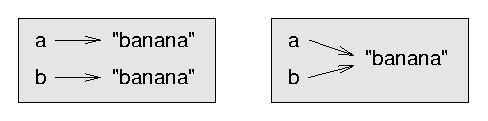
\includegraphics{illustrations/list1.eps}}
\afterfig

En un caso, \texttt{a} y \texttt{b} se refieren a cosas distintas que
tienen el mismo valor. En el segundo caso, se refieren a la 
misma cosa. Estas  ``cosas'' tienen nombres---se denominan {\bf objetos}.
Un objeto es algo a lo que se puede referir una variable.

Cada objeto tiene un  {\bf identificador} único, que podemos obtener con
la función  \texttt{id}.  Imprimiendo el identificador de \texttt{a} y \texttt{b}, 
podemos saber si se refieren al mismo objeto.

\beforeverb
\begin{verbatim}
>>> id(a)
135044008
>>> id(b)
135044008
\end{verbatim}
\afterverb
%
De hecho, obtenemos el mismo identificador dos veces, lo que nos dice
que Python sólo creó una cadena, y que  \texttt{a} y \texttt{b} se refieren
a ella.

Las listas, por otro lado, se comportan de manera diferente. Cuando
creamos dos listas obtenemos dos objetos:

\beforeverb
\begin{verbatim}
>>> a = [1, 2, 3]
>>> b = [1, 2, 3]
>>> id(a)
135045528
>>> id(b)
135041704
\end{verbatim}
\afterverb
%
\adjustpage{1}

Así que el diagrama de estados luce así:

\beforefig
\centerline{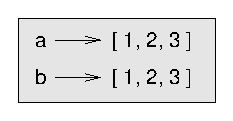
\includegraphics{illustrations/list2.eps}}
\afterfig

\texttt{a} y \texttt{b} tienen el mismo valor pero no se
refieren al mismo objeto.


\section{Alias}
\index{alias}
\index{referencia!alias}

Como las variables se pueden referir a objetos, si asignamos
una variable a otra, las dos se referirán al mismo objeto:

\beforeverb
\begin{verbatim}
>>> a = [1, 2, 3]
>>> b = a
\end{verbatim}
\afterverb
%
En este caso el diagrama de estados luce así:

\beforefig
\centerline{
\includegraphics{illustrations/list3.eps}}
\afterfig

Como la misma lista tiene dos nombres distintos, \texttt{a} y \texttt{b}, 
podemos decir que b es un {\bf alias} de a. Los cambios que se 
hagan a través de un alias afectan al otro:

\beforeverb
\begin{verbatim}
>>> b[0] = 5
>>> print a
[5, 2, 3]
\end{verbatim}
\afterverb
%
Aunque este comportamiento puede ser útil, algunas veces puede
ser indeseable. En general, es más seguro evitar los alias 
cuando se está trabajando con objetos mutables. Para objetos
inmutables no hay problema. Esta es la razón por la que
Python tiene la libertad de crear alias a cadenas cuando ve
la oportunidad de economizar memoria. Pero tenga en cuenta que esto 
puede variar en las diferentes versiones de Python; por lo tanto no es
recomendable realizar programas que dependan de este comportamiento.


\section{Clonando listas}
\index{lista!clonando}
\index{clonando}

Si queremos modificar una lista y conservar una copia de la original,
necesitamos realizar una copia de la lista, no sólo de la referencia.
Este proceso se denomina {\bf clonación}, para evitar la ambigüedad
de la palabra ``copiar''.

La forma más sencilla de clonar una lista es usar el operador segmento:

\beforeverb
\begin{verbatim}
>>> a = [1, 2, 3]
>>> b = a[:]
>>> print b
[1, 2, 3]
\end{verbatim}
\afterverb
%
Al tomar cualquier segmento de  \texttt{a} creamos una nueva lista.  En 
este caso el segmento comprende toda la lista.

Ahora podemos realizar cambios a \texttt{b} sin preocuparnos por \texttt{a}:

\beforeverb
\begin{verbatim}
>>> b[0] = 5
>>> print a
[1, 2, 3]
\end{verbatim}
\afterverb
%
\begin{quote}
{\em Como ejercicio, dibuje un diagrama de estados para \texttt{a} y \texttt{b}
antes y después de este cambio.}
\end{quote}



\section{Listas como parámetros}
\index{listas!como parámetros}
\index{parámetro}
\index{parámetro!lista}

Pasar una lista como argumento es pasar una referencia, no una copia
de ella. Por ejemplo, la función \texttt{cabeza} toma una lista como
 parámetro y retorna el primer elemento:

\beforeverb
\begin{verbatim}
def cabeza(lista):
  return lista[0]
\end{verbatim}
\afterverb
%
Se puede usar así:

\beforeverb
\begin{verbatim}
>>> numeros = [1, 2, 3]
>>> cabeza(numeros)
1
\end{verbatim}
\afterverb
%
El parámetro \texttt{lista} y la variable \texttt{numeros} son 
alias para el mismo objeto.  El diagrama de estados luce así:

\beforefig
\centerline{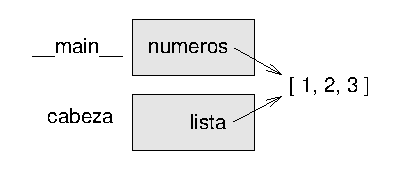
\includegraphics{illustrations/stack5.eps}}
\afterfig

Como el objeto lista está compartido por dos marcos, lo
dibujamos en el medio.

Si una función modifica un parámetro de tipo lista, el que hizo el llamado
ve los cambios. Por ejemplo, \texttt{borrarCabeza} borra el primer 
elemento de una lista:

\beforeverb
\begin{verbatim}
def borrarCabeza(lista):
  del lista[0]
\end{verbatim}
\afterverb
%
Y se puede usar así::

\beforeverb
\begin{verbatim}
>>> numeros = [1, 2, 3]
>>> borrarCabeza(numeros)
>>> print numeros
[2, 3]
\end{verbatim}
\afterverb
%
Si una función retorna una lista, retorna una referencia a ella.
Por ejemplo, la función \texttt{cola} retorna una lista que contiene 
todos los elementos, excepto el primero:

\beforeverb
\begin{verbatim}
def cola(lista):
  return lista[1:]
\end{verbatim}
\afterverb
%
\texttt{cola} se puede usar así:

\beforeverb
\begin{verbatim}
>>> numeros = [1, 2, 3]
>>> resto = cola(numeros)
>>> print resto
[2, 3]
\end{verbatim}
\afterverb
%
Como el valor de retorno se creó con el operador segmento, es una
nueva lista. La creación de  \texttt{resto}, y los cambios subsecuentes
sobre esta variable no tienen efecto sobre \texttt{numeros}.



\section{Listas anidadas}
\label{nested lists}
\index{listas anidadas}
\index{lista!anidada}

Una lista anidada aparece como elemento dentro de otra lista.
En la siguiente lista, el tercer elemento es una lista anidada:

\beforeverb
\begin{verbatim}
>>> lista = ["hola", 2.0, 5, [10, 20]]
\end{verbatim}
\afterverb
%
Si imprimimos \texttt{lista[3]}, vemos \texttt{[10, 20]}. Para 
tomar un elemento de la lista anidada podemos realizar dos pasos:

\beforeverb
\begin{verbatim}
>>> elt = lista[3]
>>> elt[0]
10
\end{verbatim}
\afterverb
%
O, los podemos combinar:

\beforeverb
\begin{verbatim}
>>> lista[3][1]
20
\end{verbatim}
\afterverb
%
Las aplicaciones del operador corchete se evalúan de izquierda a derecha, 
así que ésta expresión obtiene el elemento 3 de  \texttt{lista} y
extrae de allí el elemento 1.

\section{Matrices}
\index{matriz}
\index{lista!anidada}

Las listas anidadas se usan a menudo para representar matrices.  Por ejemplo,
la matriz:

\beforefig
\centerline{
\includegraphics{illustrations/matrix.eps}}
\afterfig

se puede representar así:

\beforeverb
\begin{verbatim}
>>> matriz = [[1, 2, 3], [4, 5, 6], [7, 8, 9]]
\end{verbatim}
\afterverb
%
\texttt{matriz} es una lista con tres elementos, cada uno es una 
fila.  Podemos seleccionar una fila de la manera usual:

\beforeverb
\begin{verbatim}
>>> matriz[1]
[4, 5, 6]
\end{verbatim}
\afterverb
%
O podemos extraer un elemento individual de la matriz usando
dos índices:

\beforeverb
\begin{verbatim}
>>> matriz[1][1]
5
\end{verbatim}
\afterverb
%
El primero escoge la fila, y el segundo selecciona la columna.
Aunque esta forma de representar matrices es común, no es la
única posibilidad. Una pequeña variación consiste en usar una 
lista de columnas en lugar de una lista de filas. Más adelante
veremos una alternativa más radical, usando un diccionario.

\index{diccionario}
\index{fila}
\index{columna}


\section{Cadenas y listas}
\index{función split}
\index{función join}

Dos de las funciones más usadas del módulo  \texttt{string} implican
listas de cadenas. \texttt{split} separa una cadena en una lista
de palabras. Por defecto, cualquier número de espacios en blanco sirven
como criterio de separación:

\beforeverb
\begin{verbatim}
>>> import string
>>> cancion = "La vida es un ratico..."
>>> string.split(cancion)
['La', 'vida', 'es', 'un', 'ratico...']
\end{verbatim}
\afterverb
%
Un argumento opcional denominado  {\bf delimitador} se puede usar
para especificar que carácteres usar como criterio de separación.
El siguiente ejemplo usa la cadena \texttt{an} como delimitador:

\beforeverb
\begin{verbatim}
>>> string.split( "La rana que canta", "an")
['La r', 'a que c', 'ta']
\end{verbatim}
\afterverb
%
Note que el delimitador no aparece en la lista resultante.

La función \texttt{join} es la inversa de \texttt{split}.  Toma 
una lista de cadenas y las concatena con un espacio entre
cada par:

\beforeverb
\begin{verbatim}
>>> m = ['La', 'vida', 'es', 'un', 'ratico']
>>> string.join(m)
'La vida es un ratico'
\end{verbatim}
\afterverb
%
Como  \texttt{split}, \texttt{join} puede recibir un argumento 
adicional separador que se inserta entre los elementos:

\beforeverb
\begin{verbatim}
>>> string.join(m, '_')
'La_vida_es_un_ratico'
\end{verbatim}
\afterverb

\begin{quote}
\begin{quote}
{\em Como ejercicio, describa la relación entre las expresiones \texttt{cadena} 
y {\tt string.join(string.split(cadena))}. ¿Son iguales
para todas las cadenas? ¿Cuando serían diferentes?}
\end{quote}
\end{quote}


\section{Glosario}

\begin{description}

\item[Lista:] colección de objetos que recibe un nombre. Cada objeto se
identifica con un índice o número entero positivo.

\item[Índice:] valor o variable entero que indica la posición de un elemento en una lista.

\item[Elemento:] uno de los valores dentro de una lista (u otra secuencia).  El 
operador corchete selecciona elementos de una lista.

\item[Secuencia:] los tipos de datos que contienen un conjunto ordenado de
elementos, identificados por índices.

\item[Lista anidada:] lista que es elemento de otra lista.

\item[Recorrido de una lista:] es el acceso secuencial de cada elemento de una lista.

\item[Objeto:] una cosa a la que una variable se puede referir.

\item[Alias:] cuando varias variables tienen referencias hacia el mismo objeto.

\item[Clonar:] crear un objeto con el mismo valor que un objeto preexistente.
Copiar una referencia a un objeto crea un alias, pero no clona el objeto.

\item[Delimitador:] carácter o cadena que se usa para indicar el lugar donde una cadena debe ser separada.

\index{lista}
\index{índice}
\index{secuencia}
\index{elemento}
\index{lista anidada}
\index{recorrido de una lista}
\index{objeto}
\index{alias}
\index{clonar}
\index{delimitador}

\end{description}
